\documentclass[12pt]{article}
\usepackage[utf8]{inputenc}
\usepackage{graphicx}
\usepackage[a4paper,width=150mm,top=25mm,bottom=25mm]{geometry}
\usepackage{float}
\usepackage[utf8]{vietnam}
\title{
{
\includegraphics[width=4.5cm, height=4.5cm]{Figs/logo-uit-300x248.png}
}
\\
{Báo Cáo Đồ Án Cuối Kì - IE303.N21.CNCL \\ Spring Movie Review}
}



\author{Hoàng Tân, Mai Anh, Quỳnh Hương \\ Giảng viên hướng dẫn: Nguyễn Văn Kiệt }

\begin{document}

\maketitle
\tableofcontents
\section{Giới thiệu đồ án}
\subsection{Tổng quan về đồ án}
Đồ án này nhằm mục đích nghiên cứu và phát triển một ứng dụng web dựa trên framework Spring Boot, được xây dựng để quản lý thông tin về phim. Ứng dụng cung cấp các tính năng cho người dùng như đề xuất, tìm kiếm, xem thông tin chi tiết, và đánh giá phim.

Mục tiêu của đồ án là tạo ra một nền tảng linh hoạt và dễ dàng mở rộng, cho phép người dùng tìm kiếm và khám phá các bộ phim dựa trên nhiều tiêu chí như thể loại, năm sản xuất, và tên phim. Đồng thời, ứng dụng cũng cung cấp tính năng đánh giá và đề xuất phim dựa trên sở thích của người dùng.

Để đạt được mục tiêu này, chúng mình sử dụng Spring Boot làm nền tảng phát triển chính, kết hợp với các công nghệ và thư viện phổ biến như PostgreSQL, Thymeleaf, Bootstrap, và Hibernate. Ứng dụng được xây dựng theo kiến trúc MVC (Model-View-Controller), giúp tách biệt logic xử lý, giao diện và dữ liệu.

Trong phần còn lại của báo cáo, chúng mình sẽ trình bày chi tiết về thiết kế và triển khai của ứng dụng, cũng như kết quả đạt được và các hướng phát triển tiềm năng.

\begin{figure}[H]
    \centering
    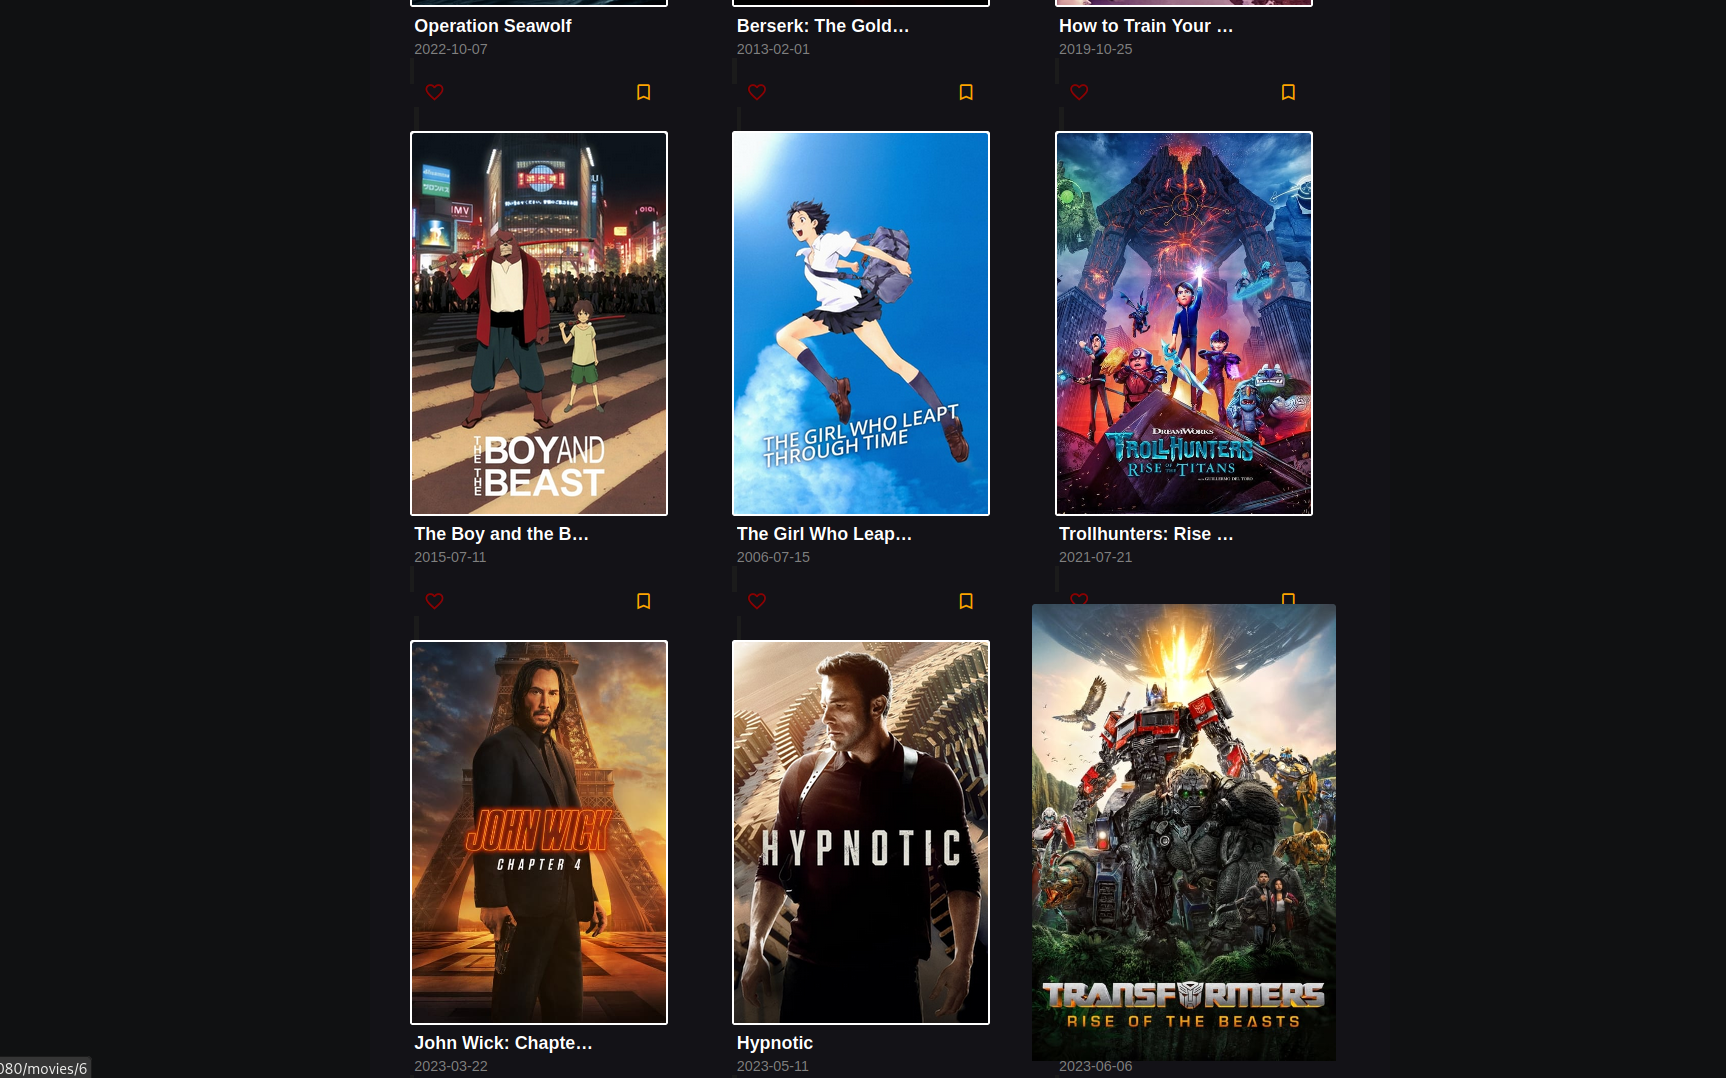
\includegraphics[scale=0.35]{Figs/Project_Review.png}
    \caption{Spring Boot Review Website}
\end{figure}
\subsection{ Đặt vấn đề}
Trong thời đại công nghệ thông tin phát triển mạnh mẽ như hiện nay, ngành công nghiệp điện ảnh đang trở thành một phần không thể thiếu của cuộc sống hàng ngày. Việc tìm kiếm và khám phá các bộ phim phù hợp với sở thích cá nhân đã trở thành một thách thức cho nhiều người.

Hiện nay, có rất nhiều nguồn thông tin về phim trực tuyến nhưng việc tìm kiếm và lọc thông tin này để tìm ra những bộ phim phù hợp và đáng xem vẫn là một vấn đề khó khăn. Người dùng thường phải dành nhiều thời gian và công sức để tìm kiếm thông tin về phim, cũng như dựa vào ý kiến của người khác để đưa ra quyết định xem phim.

Để giải quyết vấn đề này, đồ án này đề xuất một ứng dụng web quản lý thông tin về phim, cung cấp các tính năng tìm kiếm, xem thông tin chi tiết và đánh giá phim. Ứng dụng sẽ giúp người dùng dễ dàng tìm kiếm các bộ phim theo tiêu chí như thể loại, năm sản xuất và tên phim. Đồng thời, ứng dụng cũng đề xuất các bộ phim dựa trên sở thích cá nhân của người dùng, giúp họ khám phá thêm nhiều bộ phim mới và đáng chú ý.

Bằng cách áp dụng các công nghệ và công cụ phát triển phần mềm hiện đại, chúng mình hy vọng rằng ứng dụng sẽ giúp người dùng tiết kiệm thời gian và nỗ lực trong việc tìm kiếm và khám phá thế giới điện ảnh, đồng thời mang đến trải nghiệm xem phim tốt hơn.
\subsection{Ý nghĩa của đồ án}
Đồ án này mang lại nhiều ý nghĩa quan trọng từ các khía cạnh khác nhau. Dưới đây là một số ý nghĩa chính mà đồ án đem lại:
\begin{itemize}
    \item \textbf{Tiện lợi cho người dùng}: Ứng dụng web quản lý thông tin về phim sẽ mang lại tiện ích và thuận lợi cho người dùng trong việc tìm kiếm, xem thông tin chi tiết và đánh giá phim. Người dùng có thể dễ dàng tìm kiếm các bộ phim theo tiêu chí mong muốn, tiết kiệm thời gian và nỗ lực trong việc khám phá thế giới điện ảnh.
    \item \textbf{Cung cấp thông tin đa dạng về phim}: Với bộ dữ liệu với hơn \textbf{2000} phim thuộc nhiều thể loại, ứng dụng giúp người dùng tiếp cận với nhiều thể loại phim và nhiều bộ phim đáng chú ý. Điều này sẽ mở rộng khả năng khám phá và tìm kiếm các bộ phim mới, mang đến trải nghiệm xem phim đa dạng và phong phú.
    \item \textbf{Đề xuất phim dựa trên sở thích cá nhân}:  Ứng dụng sẽ sử dụng thông tin về sở thích cá nhân của người dùng để đề xuất các bộ phim phù hợp. Điều này giúp người dùng khám phá thêm nhiều bộ phim mới và đáng chú ý, mở rộng khả năng xem phim và tận hưởng những trải nghiệm mới.
    \item \textbf{Áp dụng các công nghệ phát triển phần mềm}: Đồ án này sử dụng các công nghệ và công cụ phát triển phần mềm hiện đại như Spring Boot, PostgreSQL và các thư viện phổ biến như Thymeleaf và Bootstrap. Việc áp dụng và tiếp cận các công nghệ này giúp nâng cao kỹ năng và hiểu biết về phát triển ứng dụng web.
    \item \textbf{Tiềm năng phát triển và ứng dụng trong thực tế}:Đồ án mang lại tiềm năng phát triển và ứng dụng rộng rãi trong thực tế. Các tính năng và công nghệ đã sử dụng có thể được mở rộng và tùy chỉnh để phục vụ cho các ứng dụng quản lý thông tin khác, không chỉ riêng trong lĩnh vực điện ảnh.
\end{itemize}
Qua việc thực hiện đồ án này, chúng tôi hy vọng rằng sẽ đem lại giá trị thực tiễn và đáp ứng được nhu cầu của người dùng trong việc tìm kiếm và khám phá thế giới điện ảnh một cách tiện lợi và hấp dẫn.


\subsection{ Khảo sát các công trình liên quan}
\subsubsection{Các công trình}
Trước khi triển khai đồ án, chúng mình đã tiến hành khảo sát và nghiên cứu các công trình liên quan trong lĩnh vực quản lý thông tin phim. Dưới đây là một số công trình quan trọng mà chúng tôi đã khảo sát:
\begin{itemize}
    \item \textbf{IMDb (Internet Movie Database)}: là một trong những công trình nổi tiếng và phổ biến nhất trong việc quản lý thông tin về phim trực tuyến. 
    \item \textbf{Rotten Tomatoes}: là một trang web đánh giá phim và chương trình truyền hình.
    \item \textbf{Letterboxd}: Letterboxd là một mạng xã hội cho phép người dùng tạo và chia sẻ danh sách phim yêu thích, đánh giá và nhận xét phim, và tương tác với cộng đồng người dùng khác.
    \item \textbf{Netflix, Amazon Prime, và các dịch vụ phát trực tuyến khác}: Các dịch vụ phát trực tuyến như Netflix và Amazon Prime cung cấp nền tảng quản lý thông tin phim cho người dùng. 
\end{itemize}
Thông qua việc khảo sát các công trình liên quan, chúng mình đã thu thập được nhiều thông tin và ý kiến quý giá về các tính năng, giao diện, và quản lý thông tin phim. Điều này đã giúp chúng mình xác định được những yếu tố quan trọng và đặc điểm độc đáo mà chúng mình muốn tích hợp vào đồ án của mình, từ đó nâng cao trải nghiệm người dùng và giá trị của ứng dụng.
\subsubsection{Những thiếu sót của những công trình hiện có}
Trong quá trình khảo sát và nghiên cứu các công trình liên quan, chúng mình đã nhận thấy một số điểm yếu của các website quản lý thông tin phim hiện có. Dưới đây là những điểm yếu quan trọng mà chúng mình đã rút ra từ các công trình khảo sát:
\begin{itemize}
    \item \textbf{Không có trailer phim}: Một số website không cung cấp trailer phim đi kèm với thông tin chi tiết của bộ phim. Điều này làm giảm khả năng người dùng có cái nhìn trực quan và cảm nhận về nội dung, phong cách và hiệu quả truyền đạt của phim. Thiếu trailer có thể khiến người dùng cảm thấy khó lòng đánh giá chính xác về sự hấp dẫn của một bộ phim.
    \begin{figure}[H]
        \centering
        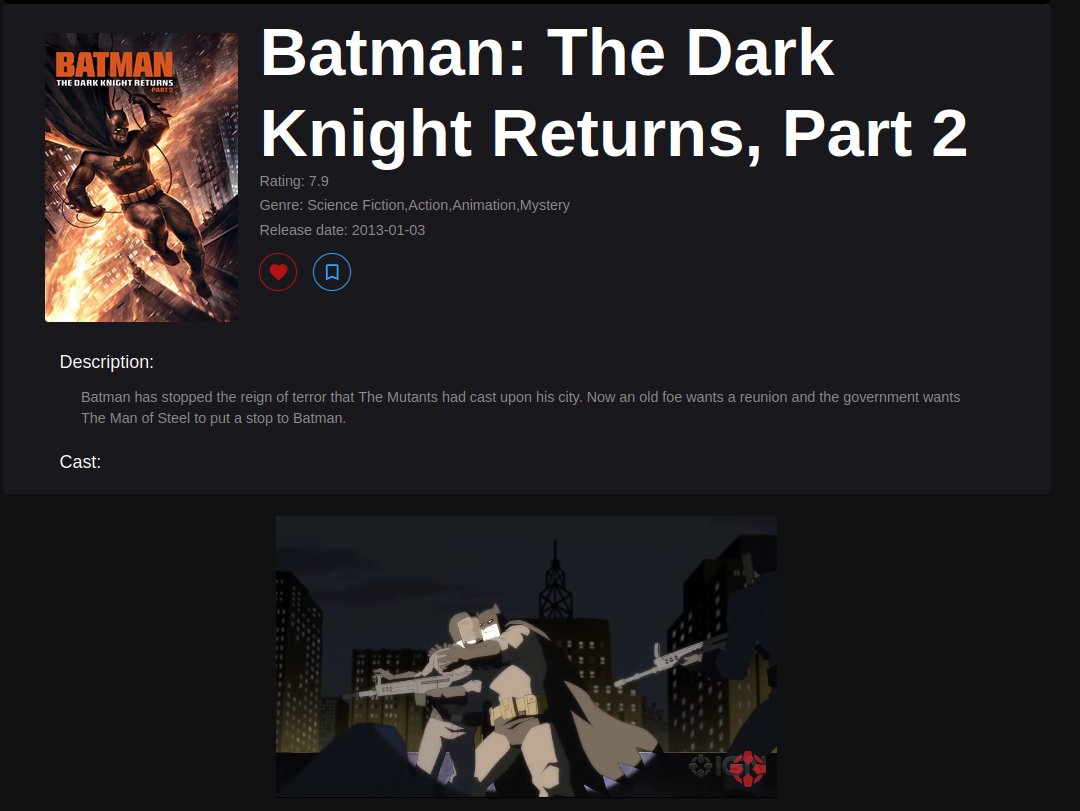
\includegraphics[scale=0.4]{Figs/Trailer_Review.png}
        \caption{Spring Movie Review hỗ trợ Trailer}
    \end{figure}
    \item \textbf{Hệ thống đánh giá không tin cậy}: Một số website có hệ thống đánh giá phim không đáng tin cậy hoặc dễ bị ảnh hưởng bởi các đánh giá không chính xác hoặc thiên vị. Điều này có thể gây ra sự bất mãn và đánh lạc hướng người dùng trong việc chọn lựa phim.
    \item \textbf{Thiếu hệ thống recommend (gợi ý)}: Một số website không có hệ thống recommend (gợi ý) phim dựa trên sở thích và lịch sử xem phim của người dùng. Điều này làm mất đi cơ hội để người dùng khám phá các bộ phim mới và đa dạng hơn, dựa trên các tiêu chí cá nhân và sở thích của họ.
\end{itemize}
Đồ án của chúng mình sẽ tập trung vào giải quyết những điểm yếu này bằng cách cung cấp trailer phim, thông tin về diễn viên (Cast) và xây dựng hệ thống recommend (gợi ý) phim thông minh, từ đó nâng cao trải nghiệm và sự hài lòng của người dùng.
\section{Lý thuyết, các công cụ sử dụng để giải quyết vấn đề}
\subsection{Lý thuyết cơ sở}

Trong phần này, chúng ta sẽ xem xét những lý thuyết cơ sở và khái niệm quan trọng liên quan đến đồ án. Những lý thuyết này cung cấp nền tảng lý thuyết và hiểu biết cần thiết để xây dựng và triển khai ứng dụng quản lý thông tin phim. Dưới đây là một số lý thuyết cơ sở quan trọng:
\begin{itemize}
    \item \textbf{Cơ sở dữ liệu quan hệ (Relational Database)}: Đồ án sử dụng cơ sở dữ liệu PostgreSQL, một hệ quản trị cơ sở dữ liệu quan hệ phổ biến. Chúng ta sẽ xem xét các khái niệm cơ bản của cơ sở dữ liệu quan hệ, bao gồm các bảng, quan hệ, khóa chính và khóa ngoại. Chúng ta cũng sẽ tìm hiểu cách sử dụng SQL để truy vấn và thao tác dữ liệu trong cơ sở dữ liệu.

    \item \textbf{Mô hình hóa dữ liệu (Data Modeling)}: Để thiết kế cơ sở dữ liệu phim, chúng mình sẽ áp dụng các nguyên tắc và kỹ thuật mô hình hóa dữ liệu. Chúng ta sẽ xem xét các mô hình dữ liệu như mô hình thực thể-liên kết và mô hình quan hệ. Chúng ta cũng sẽ tìm hiểu cách xác định các thực thể, mối quan hệ và thuộc tính trong cơ sở dữ liệu phim.

    \item \textbf{Spring Framework và Spring Boot}: Đồ án sử dụng Spring Boot, một framework phát triển ứng dụng Java nhanh chóng và dễ dùng.Tìm hiểu về các thành phần quan trọng của Spring Boot như Dependency Injection, Spring MVC, và Spring Data JPA. Tìm hiểu cách hoạt động của Spring Boot giúp chúng ta xây dựng ứng dụng web dễ dàng và hiệu quả.
    \begin{figure}[H]
        \centering
        
\includegraphics[scale=0.6]{Figs/spring-logo.png}
    \end{figure}
    \item \textbf{Mô hình phát triển MVC (Model-View-Controller)}: Ap dụng mô hình phát triển MVC để tách biệt logic xử lý, hiển thị và quản lý dữ liệu trong ứng dụng của chúng ta. Xây dựng các thành phần Model, View và Controller trong ứng dụng quản lý thông tin phim để đảm bảo tính rõ ràng, dễ bảo trì và mở rộng của mã nguồn.

\end{itemize}

Overall, the Football League Management App will provide a comprehensive solution for managing football leagues, with features designed to streamline administrative tasks, improve communication, and promote fair play and transparency.
\subsection{Các công cụ sử dụng}
Trong phần này, chúng ta sẽ tìm hiểu về các công cụ mà chúng ta sử dụng để giải quyết vấn đề trong đồ án. Các công cụ này cung cấp giải pháp và hỗ trợ cho quá trình phát triển và triển khai ứng dụng quản lý thông tin phim của chúng ta. Dưới đây là một số công cụ quan trọng mà chúng ta sử dụng:
\begin{itemize}
    \item \textbf{IntelliJ IDEA}: là môi trường phát triển tích hợp (IDE) mạnh mẽ và phổ biến dành cho phát triển ứng dụng Java. Chúng ta sử dụng IntelliJ IDEA để viết mã nguồn, quản lý dự án và thực hiện các tác vụ phát triển khác. IDE này cung cấp nhiều tính năng hữu ích như gỡ lỗi, tự động hoàn thành mã, và tích hợp với các công cụ khác.
    \begin{figure}[H]
        \centering
        
\includegraphics[scale=0.15]{Figs/IntelliJ_IDEA_Icon.svg.png}
    \end{figure}

    \item \textbf{PostgreSQL}: PostgreSQL là hệ quản trị cơ sở dữ liệu quan hệ mạnh mẽ, mã nguồn mở. Chúng mình sử dụng PostgreSQL để lưu trữ dữ liệu về phim và các thông tin liên quan. PostgreSQL cung cấp các tính năng bảo mật, khả năng mở rộng và khả năng xử lý dữ liệu phức tạp.
    \item \textbf{Thymeleaf}: Thymeleaf là một engine template đáng tin cậy và mạnh mẽ cho ứng dụng web Java. Chúng ta sử dụng Thymeleaf để tạo và hiển thị các trang HTML động trong ứng dụng. Thymeleaf kết hợp tốt với Spring Framework và cung cấp các tính năng như thực hiện biểu thức notation, lặp lại dữ liệu và binding dữ liệu.
    \item \textbf{Bootstrap}: Bootstrap là một framework CSS phổ biến và mạnh mẽ để thiết kế giao diện web responsive. Chúng mình sử dụng Bootstrap để xây dựng giao diện người dùng thân thiện và tương thích với nhiều thiết bị và kích thước màn hình khác nhau. Bootstrap cung cấp các components, lớp và kiểu patterns để tạo giao diện hấp dẫn và chuyên nghiệp.
\end{itemize}
\section{Phân tích, thiết kế, hiện thực hệ thống}
\subsection{Phân tích yêu cầu}
Trước khi tiến hành thiết kế và hiện thực hệ thống quản lý thông tin phim, chúng ta cần phân tích cẩn thận các yêu cầu chức năng và phi chức năng của đồ án. Quá trình phân tích này giúp chúng ta hiểu rõ hơn về các tính năng cần có và các yêu cầu mà hệ thống phải đáp ứng. Dưới đây là một số phân tích chính:
\subsubsection{Functional Requirements}
\begin{itemize}
    \item \textbf{Đăng nhập và đăng ký người dùng}: Cho phép người dùng tạo tài khoản và đăng nhập vào hệ thống.
    \item \textbf{Thêm, xóa, sửa phim}: Cho phép Admin có quyền thêm, xóa, sửa dữ liệu phim.
    \item \textbf{Tìm kiếm phim}: Cung cấp khả năng tìm kiếm và lọc phim dựa trên các tiêu chí như tên phim, thể loại, diễn viên, đạo diễn, năm sản xuất, v.v.
    \item \textbf{Xem chi tiết phim}: Hiển thị thông tin chi tiết về một phim cụ thể bao gồm mô tả, diễn viên, đạo diễn, thể loại, đánh giá, v.v.
    \item \textbf{Hỗ trợ Trailer phim}: Hiển thị trailer cho phim giúp người dùng có cái nhìn tổng quát về phim.
    \item \textbf{Thêm phim vào danh sách yêu thích}: Cho phép người dùng thêm phim vào danh sách yêu thích của họ để theo dõi và truy cập nhanh vào những phim mà họ quan tâm.
    \item \textbf{Tính năng Recommend phim}: Sử dụng các thuật toán để đánh giá và đề xuất những phim mà người dùng thích, Hiển thị những phim phù hợp với từng đối tượng người dùng.
    \item \textbf{Đánh giá phim}: Cho phép người dùng xem và đọc những đánh giá do người dùng khác thực hiện, cung cấp hệ thống chấm điểm cho từng phim.
\end{itemize}
\subsubsection{Non-Functional Requirements}
Ngoài các chức năng chính, chúng ta cũng cần xem xét các yêu cầu phi chức năng mà hệ thống cần đáp ứng. Điều này có thể bao gồm:
\begin{itemize}
    \item \textbf{Bảo mật}: Đảm bảo rằng chỉ người dùng đã đăng nhập mới có thể truy cập vào các chức năng và thông tin nhạy cảm.
    \item \textbf{Tính khả dụng}: Hệ thống phải có thời gian phản hồi nhanh chóng và khả năng xử lý đồng thời nhiều yêu cầu từ người dùng.
    \item \textbf{Giao diện người dùng thân thiện}: Thiết kế giao diện người dùng đơn giản, dễ sử dụng và thân thiện để người dùng có trải nghiệm tốt khi sử dụng hệ thống.
\end{itemize}
\subsubsection{Use Case Diagram}
Use case là một công cụ quan trọng trong phân tích yêu cầu. Chúng ta xác định các use case chính và các tác nhân liên quan, đồng thời xác định các tương tác giữa tác nhân và hệ thống. Use case giúp chúng ta hiểu rõ hơn về cách người dùng sẽ sử dụng hệ thống và cung cấp cơ sở cho việc thiết kế hệ thống.
\begin{figure}[H]
    \centering
    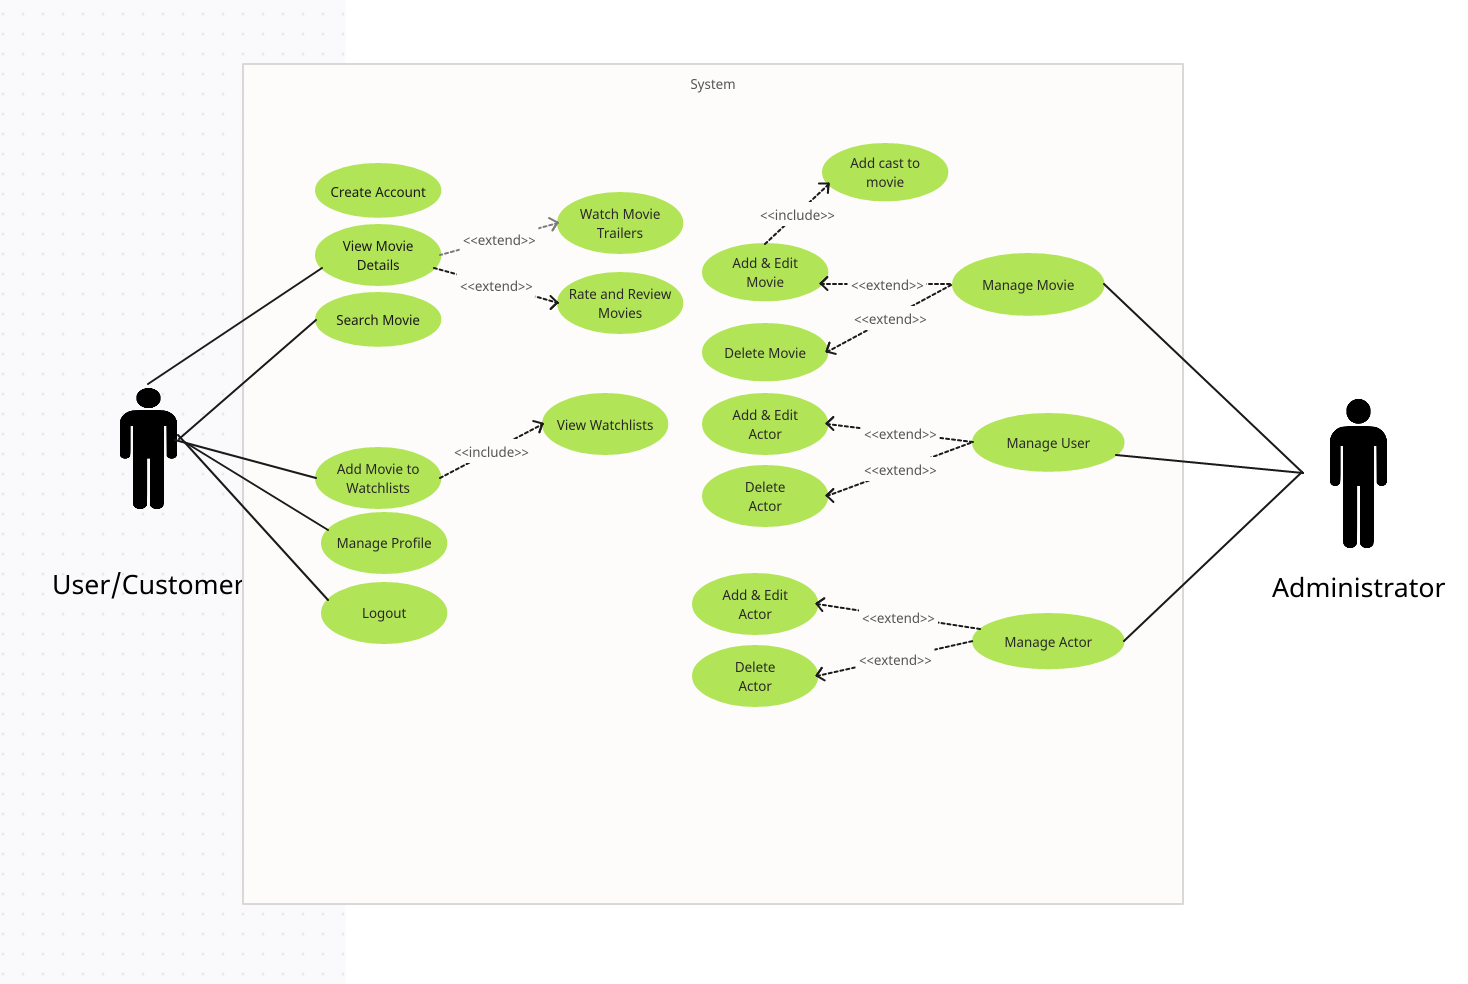
\includegraphics[scale=0.45]{Figs/Use_case.png}
    \caption{Spring Movie Review - Use Case Diagram}
\end{figure}
\end{document}
